%\section{Drone movement}\label{s:drone_movement}
In order to make a transfer function for the drone it is needed to examine how the drone behaves when it moves around. To make it simple the drone is set to only move in z-axis also known as yaw axis \ref{fig:z_axis}.
\begin{figure}[H]
    \centering
    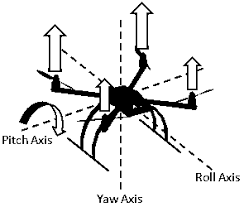
\includegraphics[width=0.45\textwidth]{figures/ch_movement/z-axis.png}
    \caption{Illustration of \cite{drone_axis}}
    \label{fig:z_axis}
\end{figure}


 As mentioned in the requirement specification \ref{sec:req}, the drone should keep a fixed distance to the floor. To be able to control the drone in the z-axis, a model for the drone will be determined. This model describing how the drone corresponds to controller inputs. The position on the z-axis is controlled by the throttle on the remote controller. The throttle values is set from 1000\% - 2000\%, where the drone is idle at 1000\% and maximum velocity at 2000\%.  

\section{Vicon}\label{s:vicon}
To determine the behaviour of the drone, it is important to know how the the drone response to the remote controller. 
Because the models are of a drone, driven by a flight controller with an unknown control system, it seems inaccessible to derive the models analytically. Instead, by measuring either an impulse response or a step
response in the z axis, the models can be determined experimentally. For this a motion tracker system, for tracking the positions of the drone. A motion tracker system called vicon is available at the university laboratory. 

\section{Transfer function for the movements}\label{s:transfer_function}
To get a model of the drone, it is needed to get a transfer function for the drones movements. To get the transfer function, a model of the drone's movements is needed, to get these data the system Vicon is used. The data that is needed is for a step response, this step response will only be for the z-axis. When this step response is plotted it gives a function, this function will be use to make the transfer function. This function is called h(s)
that depends on the input and output of the function. All these functions depends on the time. To get a better view of have this transfer function works can be seen on the figure \ref{fig:transfer_function}.
\begin{figure}[H]
    \centering
    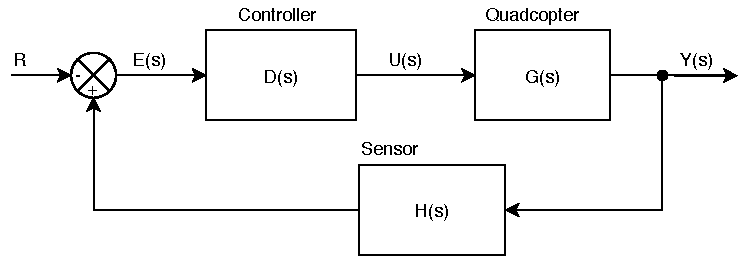
\includegraphics[width=0.75\textwidth]{figures/ch_design/transfer_function.pdf}
    \caption{An illustration of the transfer diagram}
    \label{fig:transfer_function}
\end{figure}

From this diagram it can be seen that the transfer function is applied an unit step $\frac{1}{s}$. 






